% Beamer Presentation using LaTeXas theme
% author: Joshua E. Hammond
% date: March 21, 2023

% to show layout:
% imports
% \documentclass{beamer}  % 4:3 ratio by default 
% notes from how it's defined:
% papersize={12.8cm,9.6cm},
% hmargin=1cm,%
% vmargin=0cm,%
% head=0.5cm,% might be changed later
% headsep=0pt,%
% foot=0.5cm% might be changed later
\documentclass[aspectratio=169]{beamer}  % 16:9 ratio
% notes from how it's defined:
% papersize={16.00cm,9.00cm},
% hmargin=1cm,%
% vmargin=0cm,%
% head=0.5cm,% might be changed later
% headsep=0pt,%
% foot=0.5cm% might be changed later

% \usepackage[showframe]{geometry}
% \usepackage{layout}
% \usepackage{framed}
% \usepackage{graphicx}

\usepackage[utf8]{inputenc}
\hypersetup{pdfpagemode=FullScreen}  % open as full page by default

\usepackage[export]{adjustbox}
\usepackage{array}

\usepackage{caption} % used so figures dont have "figure#: " prefix
\captionsetup[figure]{labelformat=empty}

\usepackage{manyfoot} 

\usepackage[backend=biber,style=numeric-comp,sorting=none, maxbibnames=99,maxcitenames=1]{biblatex}
\AtEveryCitekey{\clearfield{url}}  % removes url as citations happen to reduce space taken on slides

% macro for footnote without marker
\makeatletter
\def\blfootnote{\xdef\@thefnmark{}\@footnotetext}
\makeatother

\usetheme{LaTeXas}

% define parameters
\title[Short Title]{Optimization Under Uncertainty for Decarbonization} 
\subtitle{}

\author[Hammond]{Joshua Hammond, Michael Baldea and Brian Korgel}
\institute{McKetta Departament of Chemical Engineering}
\date{Supergroup March 22, 2023}  % date accepts short and long forms, and could include name and date of the event
% \logo{\includegraphics[]{}}  % logo generally in bottom right

%% for multi-author and showing affiliations
% \author[shortname]{author1 \inst{1} \and author2 \inst{2}}
% \institute[shortinst]{\inst{1} affiliation for author1 \and %
%                       \inst{2} affiliation for author2}

\addbibresource{refs.bib}

% document
\begin{document}

\frame[plain]{  % plain removes the footline from the title page
    \titlepage
}

\frame{
\frametitle{Outline}
\tableofcontents  % [pausesections]
}

\section{Context}
\frame{
    \frametitle{A Renewable Energy Renaissance}
    \begin{minipage}{0.5\textwidth}
        \includegraphics[width=6 cm]{assets/images/wind+solar.jpg}
    \end{minipage} \hfill
    \begin{minipage}{0.49\textwidth}
        The Biden administration has published goals for a carbon-free electric grid by 2035\footnotemark[1] and net-zero emissions by 2050\footnotemark[2].
    \end{minipage}
    \footnotetext[1]{\fullcite{whitehouse2021a}} 
    \footnotetext[2]{\fullcite{whitehouse2021b}}
}

\frame{
\frametitle{Intermittent Renewables Predominate Generation}
A 90\% clean grid is achievable today with low incremental cost. In 142 possible future scenarios studied by NREL, wind and solar provide 60\%-80\% of least-cost generation\footnotemark[1]% \footfullcite{denholm2022}.\\
\vspace{-0.2 cm}
\begin{columns}[c]
    \begin{column}{0.49\textwidth}
        \begin{figure}
        \includegraphics[width=0.95\textwidth]{assets/images/US_Annual_GHI.jpg}
        \caption{Annual U.S. Solar Potential\footnotemark[2]% \footfullcite{sengupta2018}}
        }
        \end{figure}
    \end{column}
    \begin{column}{0.49\textwidth}
        \begin{figure}
        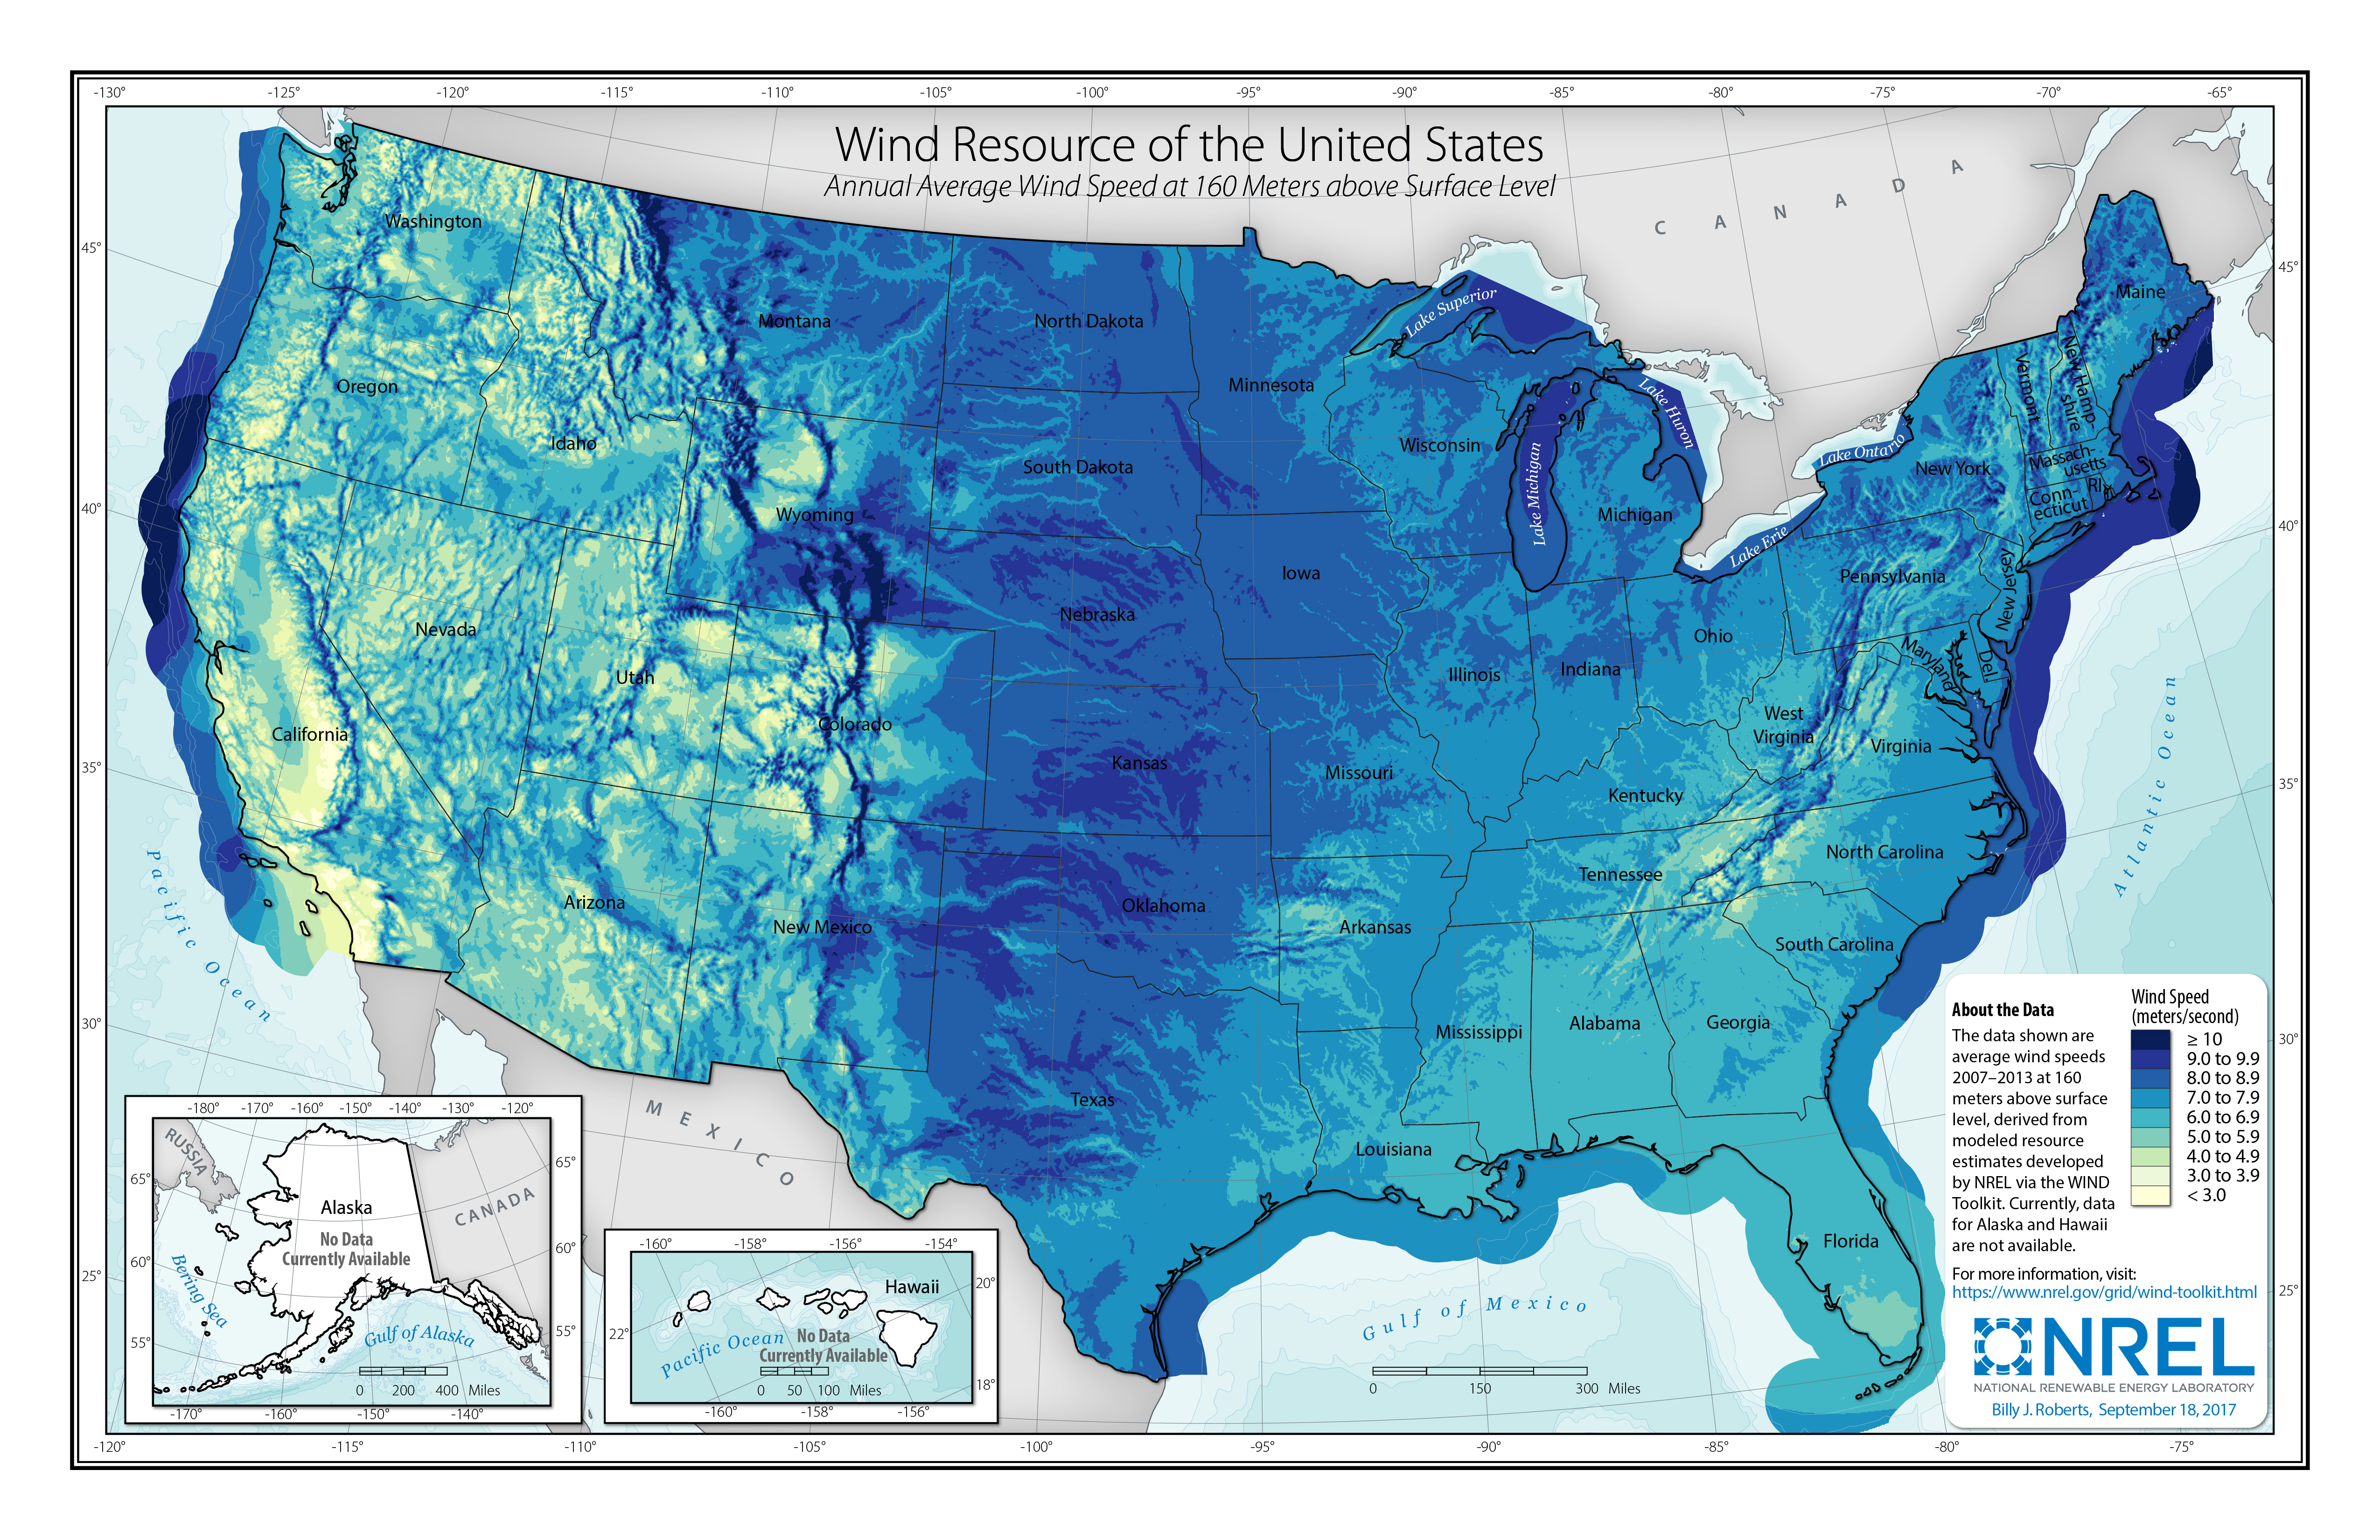
\includegraphics[width=0.95\textwidth]{assets/images/US_wind_potential.jpg}
        \caption{U.S. Wind Potential\footnotemark[3]% \footfullcite{draxl2015}}
        }
        \end{figure}
    \end{column}
\end{columns}
\vspace{-5 pt}
\footnotetext[1]{\fullcite{denholm2022}} 
\footnotetext[2]{\fullcite{sengupta2018}}
\footnotetext[3]{\fullcite{draxl2015}}
}

% \frame{
% \frametitle{Salient Disparities With the Current Grid}
% \begin{figure}
%     \centering
%     \includegraphics[height=6 cm]{assets/images/LLNL_Energy_2021.png}
%     \caption{2021 Energy Generation and Consumption\footnotemark[1]}
%     \label{fig:my_label}
% \end{figure}
% \vspace{-5 pt}
% \footnotetext[1]{\fullcite{aeo2021}}
% }

\frame{
 \frametitle{Thesis}
Current power infrastructure dispatches generation based on what load is anticipated to be.\\

\vspace{0.6 cm}

In contrast, and low-carbon future must anticipate \underline{both future load and generation}, and subsequently either shift load or dispatch stored energy to match the two.
% \begin{itemize}
%     \item Day-to-day operation and energy dispatch
%     \item Design and sizing of renewable energy and storage
% \end{itemize}
} 

\frame{
    \frametitle{Problem Statement}
    We will consider an industrial energy consumer with onsite solar power and storage. We will minimize \textbf{costs} and \textbf{scope 2 carbon emissions} by manipulating:
    \begin{itemize}
        \item<2-> When operations are scheduled
        \item<3-> How much power is dispatched to/from the grid at any given time
        \item<4-> How much power is stored or dispatched at any given time
        \item<5-> The sizing and type of local generation and energy storage
    \end{itemize}
    \vspace{-5 pt}
    \begin{figure}
        \centering
        \includegraphics<1>[height=4 cm]{assets/images/power icons/Slide1.PNG}
        \includegraphics<2>[height=4 cm]{assets/images/power icons/Slide2.PNG}
        \includegraphics<3>[height=4 cm]{assets/images/power icons/Slide3.PNG}
        \includegraphics<4>[height=4 cm]{assets/images/power icons/Slide4.PNG}
        \includegraphics<5>[height=4 cm]{assets/images/power icons/Slide5.PNG}
    \end{figure}
}

\section{Outline}
\frame{
 \frametitle{Outline}
\begin{enumerate}
    \item<1-> Anticipate future generation
    \begin{itemize}
        \item \textcolor<5>{green}{2-hours ahead} \uncover<5>{  \textcolor{green}{(Completed)}}
        \item \textcolor<5>{yellow}{Day-ahead} \uncover<5>{  \textcolor{yellow}{(In progress)}}
    \end{itemize}
    \item<2-> \textcolor<5>{teal}{Anticipate future conditions within ERCOT \uncover<5>{  (Planned)}}
    \item<3-> \textcolor<5>{teal}{Integrate models to minimize both costs and scope 2 carbon emissions \uncover<5>{  (Planned)}}
    \begin{itemize}
        \item \textcolor<5>{teal}{Process models (seperations, reactions, heating and cooling)}
        \item \textcolor<5>{teal}{Real-time operation and energy dispatch}
        \item \textcolor<5>{teal}{Coupled design and operation}
    \end{itemize}
\end{enumerate}

\uncover<4->{
\vspace{0.5 cm}
\textcolor{red}{\textbf{Optimal control \textif{anticipates} and accounts for what \underline{will happen} rather than than only what \underline{has happened}}}
}
}

\section{Completed Work}
\subsection{Intra-day Solar Irradiance Forecasting}
\frame{
    \frametitle{2 Hour-ahead Irradiance Forecasting with Skycamera}
    Accurate short-term forecasts ramp-rate control and better real-time market operation.
    \vspace{0.25 cm}
    \begin{columns}
        \begin{column}[t]{0.49\textwidth}
            Steep power ramps cause issues for load and generation balancing\\
            \begin{figure}
            \centering
            \includegraphics[width=\textwidth]{assets/images/NREL_Irradiance_Measurements.png}
            \end{figure}
        \end{column}

        \begin{column}[t]{0.49\textwidth}
            Generation is often located in remote locations with limited internet connectivity\\
            \begin{figure}
            \centering
            \includegraphics[width=\textwidth]{assets/images/desert sunlight.jpg}
            \end{figure}
        \end{column}

    \end{columns}
}

\frame{
    \frametitle{Problem Statement}
    The best short-term models for irradiance forecasting must transmit images from data-transmission limited environments. We create a model that accurately forecast irradiance up to two hours ahead while requiring less data transmission.

    \begin{figure}
        \centering
        \includegraphics[width=\textwidth]{assets/images/Tabular Inputs.png}
    \end{figure}
}

\frame{
    \frametitle{CNN-LSTM Model Extracts Temporal Patterns}
    \begin{figure}
        \centering
        \includegraphics<1>[width=0.97\textwidth]{assets/images/data transformation/Slide1.png}
        \includegraphics<2>[width=0.97\textwidth]{assets/images/data transformation/Slide2.png}
        \includegraphics<3>[width=0.97\textwidth]{assets/images/data transformation/Slide3.png}
        \includegraphics<4>[width=0.97\textwidth]{assets/images/data transformation/Slide4.png}
    \end{figure}
}

\frame{  % Redo this figure for a more vertical orientation: 14 x 7.5 cm
    \frametitle{Experimental Design}
    \begin{figure}
        \centering
        \includegraphics[width=0.99\textwidth]{assets/images/Experimental Design.png}
    \end{figure}
}

\frame{  
    \frametitle{Experiment 1: Time and Target Variable}
    Existing literature has not studied how representation of \underline{time} and \underline{future irradiance} affect the model ability to capture underlying dynamics.\\
    \vspace{0.5 cm}
    \begin{columns}
        \begin{column}[t]{0.4\textwidth}
        \textbf{Time Representation}
        \begin{itemize}
            \item Time of Day (ToD)
            \item Time of Year (ToY)
            \item Time Milestones (TM) - time from sunrise, solar noon, sunset
            \item Permutations of these
            \item Sine and Cosine Transforms of each of these
        \end{itemize}
        \end{column}
        
        \begin{column}[t]{0.59\textwidth}
        \textbf{Future Irradiance Representation} $\{I_{t+10} \cdots I_{t+120}\}$
        \begin{itemize}
            \item Scalar Irradiance $I_i$
            \item Clear Sky Index $\frac{I_i}{CS_i}$
            \item Clear Sky Difference $I_i-CS_i$
            \item Change in Irradiance $I_i - I_0$
            \item Change in Clear Sky Index $\frac{I_i}{CS_i} - \frac{I_0}{CS_0}$
        \end{itemize}
        \end{column}
    \end{columns}
    \blfootnote{Clear Sky (CS) Irradiance is the ideal Irradiance based on location, and time that does not account for weather effects}
}

\frame{
    \frametitle{Experiment 1 Results}

    \begin{columns}
        \begin{column}{0.35\textwidth}
        \begin{itemize}
            \item \textbf{Time of Day} and \textbf{Time of Year} best represent time compared to more sophisticated representations
            \item Relative representations of irradiance such as \textbf{change in clear sky index} better capture underlying weather dynamics
        \end{itemize}
        \end{column}

        \begin{column}{0.65\textwidth}
            \begin{figure}
                \centering
                \includegraphics[width=0.9\textwidth]{assets/images/Target_variables.png}
            \end{figure}
        \end{column}
    \end{columns}
    \blfootnote{Forecast skill score measures performance relative to a naive persistence forecast. Forecast skill score is calculated as $1-\frac{\text{Model Error}}{\text{Reference Error}}$. In this study we use the persistence of cloudiness model as a reference which assumes future irradiance will remain the same relative to the clear sky irradiance.}
}

\frame{  % resize figure
    \frametitle{Experiment 2: Input Time Required}
    Interestingly, error increases as more input data is provided.
    \begin{figure}
        \centering
        \includegraphics[width=0.8\textwidth]{assets/images/MAE_Time.png}
    \end{figure}
}

\frame{  % resize figure
    \frametitle{Experiment 3: Feature Importance}
    A feature permutation test\footnotemark importance demonstrates that cloud \% and historical irradiance are the largest contributors to model inference accuracy.
    \begin{figure}
        \centering
        \includegraphics[width=0.7\textwidth]{assets/images/Feature_importance.png}
    \end{figure}
    \footnotetext{Observes the increase in model prediction error when corrupting a specific column associate with that feature. While this provides an idea of the importance of certain features, it is dependent on the model, and the random shuffling involved in the column corruption.}
}

\frame{  % resize figure
    \frametitle{Final Model Evaluation}
    Our model achieves a lower accuracy than those reported by Feng et. al.\footfullcite{Feng2022}\footfullcite{Feng2020} and Al-laham et. al.\footfullcite{Al-Lahham2020d}, however our model does not require sequences of full images: only a few bytes of information are required.
    \vspace{-.3 cm}
    \begin{figure}
        \centering
        \includegraphics[width=0.7\textwidth]{assets/images/Accuracy_w_literature.png}
    \end{figure}
}

\frame{
    \frametitle{Intraday-Tabular Forecasting Key Findings}
    \begin{itemize}
        \item Future work should represent time as \textbf{time of day} and \textbf{time of year}.
        \item Future work should represent future irradiance as \textbf{change in clear sky index} as this normalizes for daily seasonality and includes an assumption of persistence
        \item Future irradiance predictions are largely dependent on current conditions rather than past data
        \item Permutation feature importance suggests those interested in short-term forecasting at a new site should only install a sky-camera and irradiance measurement equipment for minimal capital costs
    \end{itemize}
}

\subsection{Probabilistic Day-ahead Net Load Forecasting}
\frame{
    \frametitle{Net Load is Increasingly Important With Renewables}
    Net Load = Demand - Renewable Generation\\
    \begin{figure}
        \centering
        \includegraphics<1>[width=0.8\textwidth]{assets/images/Duck Curve.png}
        \includegraphics<2>[width=0.8\textwidth]{assets/images/Duck Duck Curve.png}
    \end{figure}
}

\frame{
    \frametitle{Approach}
    \begin{quote}
        Despite recent improvements in NWP, forecasts of surface solar irradiance, uncertain initial conditions, unresolved atmospheric phenomenons, complex local orography, propagation of numerical errors and approximations combine and, \textbf{in most cases, even state-of-the-art NWP models remain relatively inaccurate. Their errors, nevertheless, may be somewhat systematic and often exhibit patterns that can be learned.}
    \end{quote}
\blfootnote{\fullcite{verbois2022}}
}

\frame{
    \frametitle{Approach}
    We will be given a small amount of net-load for 34 residential distribution nodes across the U.S. and tasked with predicting the probabilistic day-ahead net load.
    \begin{enumerate}
        \item<2->Use historical net loads to find what the ideal generation is
        \item<2->Use ensembles of NREL home models fit to historical data to approximate future performance
    \end{enumerate}
    \uncover<3->{This will be a novel integration of these physics-based generation and demand models to predict net load rather than using purely statistical models}
}

% \section{Future Work}

% \frame{
%     \frametitle{Future ERCOT Scenarios}

% }

% \frame{
%     \frametitle{Optimal Operation}

% }

% \frame{
%     \frametitle{Coupled Design and Operation}

% }

\section{Review}

\frame{
    \frametitle{Review}
    \begin{enumerate}
    \item Anticipate future generation
    \begin{itemize}
        \item \textcolor{green}{2-hours ahead}  \textcolor{green}{(Completed)}
        \item \textcolor{yellow}{Day-ahead}  \textcolor{yellow}{(In progress)}
    \end{itemize}
    \item \textcolor{teal}{Anticipate future conditions within ERCOT  (Planned)}
    \item \textcolor{teal}{Integrate models to minimize both costs and scope 2 carbon emissions \uncover{  (Planned)}}
    \begin{itemize}
        \item \textcolor{teal}{Process models (seperations, reactions, heating and cooling)}
        \item \textcolor{teal}{Real-time operation and energy dispatch}
        \item \textcolor{teal}{Coupled design and operation}
    \end{itemize}
\end{enumerate}
\begin{figure}
    \centering
    \includegraphics[width=0.45\textwidth]{assets/images/power icons/Slide5.PNG}
    \caption{Caption}
    \label{fig:my_label}
\end{figure}

}

\frame{
    \frametitle{Thanks}
    \begin{figure}
        \centering
        \includegraphics[width=0.6\textwidth]{assets/images/Baldea_group.png}
        \includegraphics[width=0.6\textwidth]{assets/images/Korgel_group.jpg}
    \end{figure}
}

\section{Questions}

\frame{
    \frametitle{Questions?}
    \begin{enumerate}
    \item Anticipate future generation
    \begin{itemize}
        \item \textcolor{green}{2-hours ahead}  \textcolor{green}{(Completed)}
        \item \textcolor{yellow}{Day-ahead}  \textcolor{yellow}{(In progress)}
    \end{itemize}
    \item \textcolor{teal}{Anticipate future conditions within ERCOT  (Planned)}
    \item \textcolor{teal}{Integrate models to minimize both costs and scope 2 carbon emissions \uncover{  (Planned)}}
    \begin{itemize}
        \item \textcolor{teal}{Process models (seperations, reactions, heating and cooling)}
        \item \textcolor{teal}{Real-time operation and energy dispatch}
        \item \textcolor{teal}{Coupled design and operation}
    \end{itemize}
\end{enumerate}
\begin{figure}
    \centering
    \includegraphics[width=0.45\textwidth]{assets/images/power icons/Slide5.PNG}
    \caption{Caption}
    \label{fig:my_label}
\end{figure}
}

\section{Supplemental Material}

\frame{
    \frametitle{Pivot Table: Time and Target Representation}

    % \begin{table}
    % \centering
    % \caption{Mean Absolute Error for Experiment 1. Each row represents a different way of representing time and each column represents the a different representation of future irradiance}
    % \begin{tabular}{lrrrrr}
    % \toprule
    % {} &  $\Delta$ CSI &  $\Delta$ I &  CS Dev. &    CSI &      I \\
    % \midrule
    % \textbf{$\angle$ TM                            } &        108.20 &      106.61 &   106.36 & 108.76 & 117.58 \\
    % \textbf{$\angle$ ToD                           } &        109.37 &      112.00 &   106.19 & 108.01 & 114.53 \\
    % \textbf{$\angle$ ToD, $\angle$ TM              } &        109.35 &      106.71 &   107.80 & 110.61 & 116.21 \\
    % \textbf{$\angle$ ToD, $\angle$ ToY             } &        111.27 &      110.86 &   109.15 & 109.38 & 114.77 \\
    % \textbf{$\angle$ ToD, $\angle$ ToY, $\angle$ TM} &        108.96 &      108.14 &   109.05 & 110.83 & 114.66 \\
    % \textbf{$\angle$ ToY                           } &        109.34 &      108.51 &   107.42 & 112.55 & 112.78 \\
    % \textbf{$\angle$ ToY, $\angle$ TM              } &        181.75 &      197.71 &   107.71 & 109.86 & 113.18 \\
    % \textbf{TM                                     } &        107.15 &      110.19 &   109.26 & 109.80 & 114.31 \\
    % \textbf{ToD                                    } &        110.71 &      113.16 &   108.44 & 111.56 & 115.10 \\
    % \textbf{ToD, TM                                } &        \textbf{106.00} &      109.54 &   111.13 & 112.15 & 112.99 \\
    % \textbf{ToD, ToY                               } &        106.08 &      288.77 &   112.25 & 106.85 & 110.64 \\
    % \textbf{ToD, ToY, TM                           } &        174.73 &      109.25 &   107.92 & 108.33 & 117.24 \\
    % \textbf{ToY                                    } &        108.19 &      435.81 &   110.16 & 112.81 & 111.95 \\
    % \textbf{ToY, TM                                } &        111.48 &      110.17 &   108.65 & 110.10 & 112.97 \\
    % \bottomrule
    % \end{tabular}
    % \end{table}
}

% \frame{
%     \frametitle{References}
%     \bibliographystyle{ieeetr}
%     \printbibliography
% }

\end{document}
